
\section{Project Structure Overview:}

The Breadit project is structured as a monorepo utilizing npm workspaces. This architecture decouples the frontend client interface, backend server logic, and shared utility definitions, allowing independent component lifecycle management, easier deployment containerization, and unified types across the platform.
\begin{figure}[H]
  \centering
  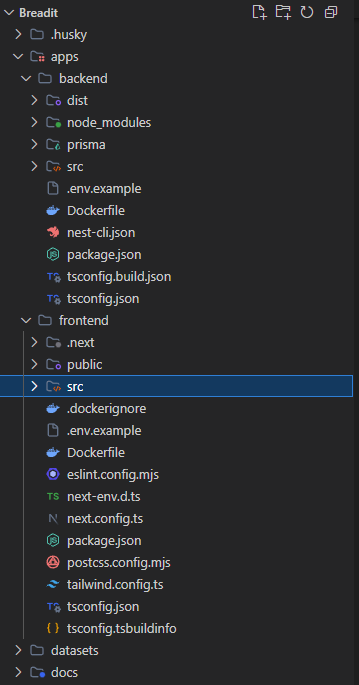
\includegraphics[width=0.92\linewidth,height=0.82\textheight,keepaspectratio]{images/image36.png}
  \caption{Project Structure}
  \label{fig:30}
\end{figure}

\section{Backend Implementation}

The backend functionality of Breadit is developed using the NestJS framework built on top of Fastify for high-performance HTTP request handling and WebSocket communication. The server interacts with a PostgreSQL database using Prisma ORM to manage data persistence and type safety across database operations.

\subsection{Database Models}

The system's data layer architecture is centrally defined in the schema.prisma file. This configuration file houses declarative schema models that Prisma translates into relational database tables and TypeScript interfaces.
\begin{figure}[H]
  \centering
  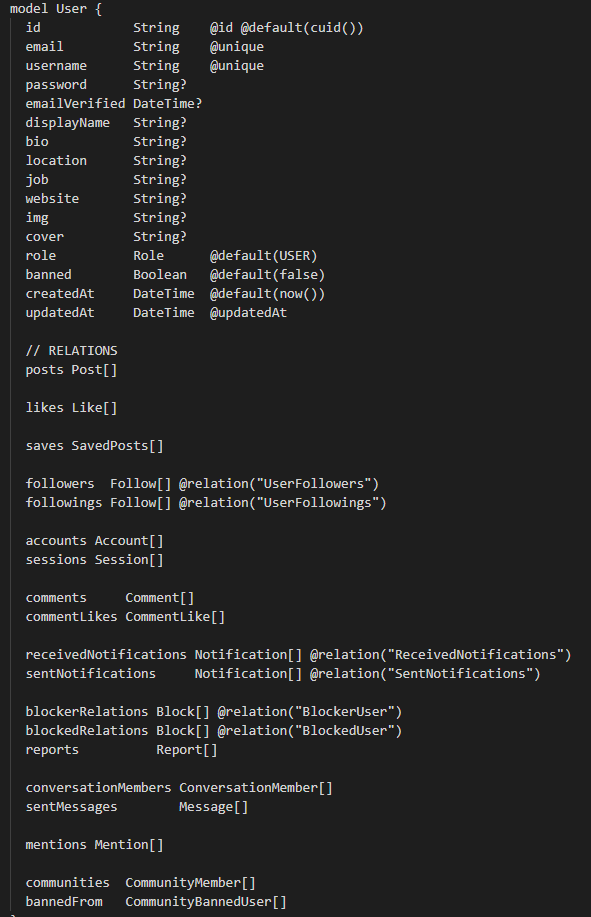
\includegraphics[width=0.92\linewidth,height=0.82\textheight,keepaspectratio]{images/image37.png}
  \caption{Code Snippet -- SiteUser Model Definition}
  \label{fig:31}
\end{figure}

\subsection{Module 1: Authentication \& Account Verification}

\textbf{Controller }\textbf{(API}\textbf{ }\textbf{routes)}\textbf{:} Exposes RESTful endpoints for authentication. It integrates NestJS @Throttle decorators to enforce rate-limiting rules (maximum of 10 requests per 60 seconds) at the entry layer, protecting sensitive operations like Registration, Login, and OTP Verification from automated dictionaries and brute-force attacks.
\begin{figure}[H]
  \centering
  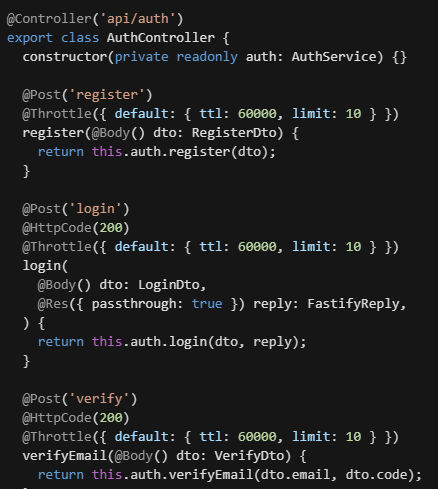
\includegraphics[width=0.92\linewidth,height=0.82\textheight,keepaspectratio]{images/image38.png}
  \caption{Code Snippet -- Authentication \& Account Verification}
  \label{fig:32}
\end{figure}

\textbf{Service (Business Logic)}: Implements secure password verification using bcrypt.compare against hashed credentials stored in PostgreSQL. Upon successful authentication, it generates stateless JSON Web Token (JWT) using the jose library containing the user session claims. This JWT is appended to the Fastify response header via a secure, httpOnly, sameSite: 'lax' cookie, shielding the application from Cross-Site Scripting (XSS) token interception.
\begin{figure}[H]
  \centering
  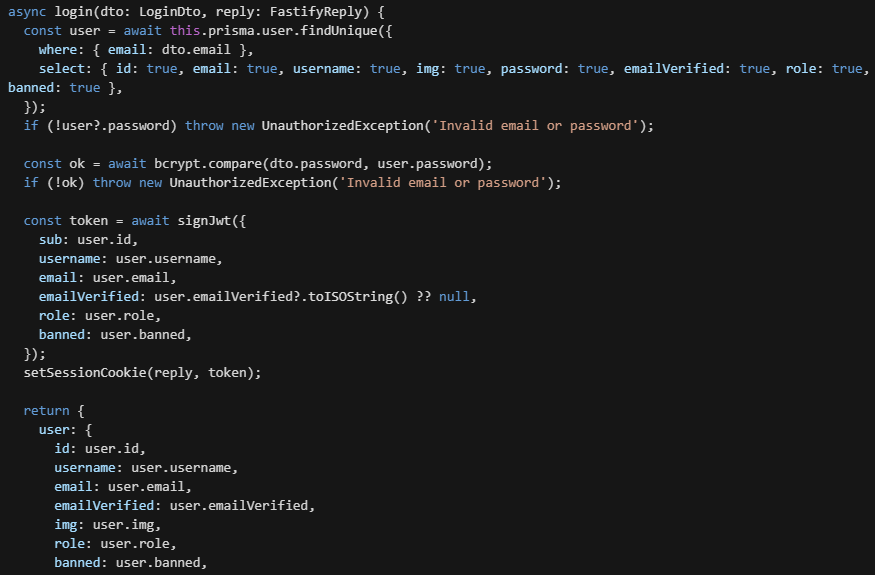
\includegraphics[width=0.92\linewidth,height=0.82\textheight,keepaspectratio]{images/image39.png}
  \caption{Code Snippet -- Authentication \& Account Verification}
  \label{fig:33}
\end{figure}

\subsection{Module 2: Feeds \& Discovery}

\textbf{Controller (API Routes):} Handlers request for dynamic feed retrieval. It utilizes an OptionalJwtAuthGuard to determine session presence: if the request is authenticated, the client is identified (req.user.id) to fetch personalized interactions (such as like and bookmark statuses); if anonymous, the request bypasses session enforcement to serve generic public feeds.
\begin{figure}[H]
  \centering
  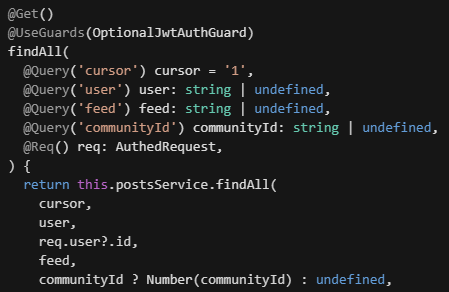
\includegraphics[width=0.92\linewidth,height=0.82\textheight,keepaspectratio]{images/image40.png}
  \caption{Code Snippet -- Feed \& Discovery}
  \label{fig:34}
\end{figure}

\textbf{Service (Business Logic \& Algorithm):} Implements a time-decay explore feed ranking algorithm. The system aggregates dynamic user signals (likes, comments, reposts) and applies a linear decay factor based on post age (ageHours). It further applies a diversity filter (applyExploreDiversity) that limits consecutive posts from the same author to 3, ensuring feed variety and preventing monopoly of the explore feed by single active users.
\begin{figure}[H]
  \centering
  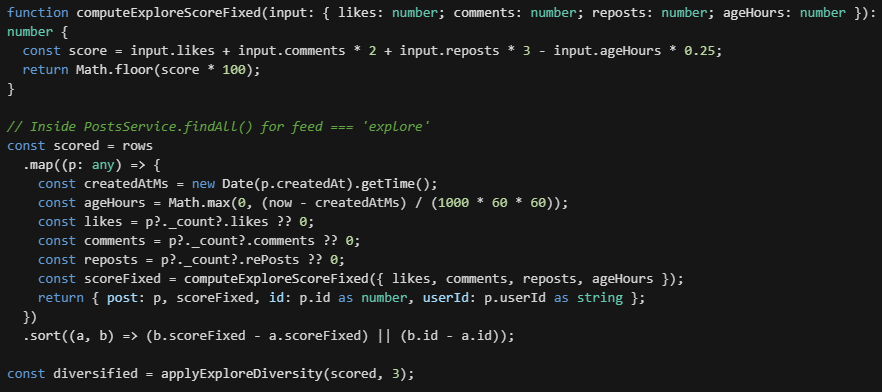
\includegraphics[width=0.92\linewidth,height=0.82\textheight,keepaspectratio]{images/image41.png}
  \caption{Code Snippet -- Feed \& Discovery}
  \label{fig:35}
\end{figure}

\subsection{Module 3: Post Management}

\textbf{Controller (API Routes):} Handles post creation requests submitted via multipart/form-data. Because the project runs on Fastify instead of Express, file uploads are processed asynchronously using non-blocking streams (req.parts()), which significantly reduces memory utilization and avoids high-RAM spikes during concurrent heavy file uploads.
\begin{figure}[H]
  \centering
  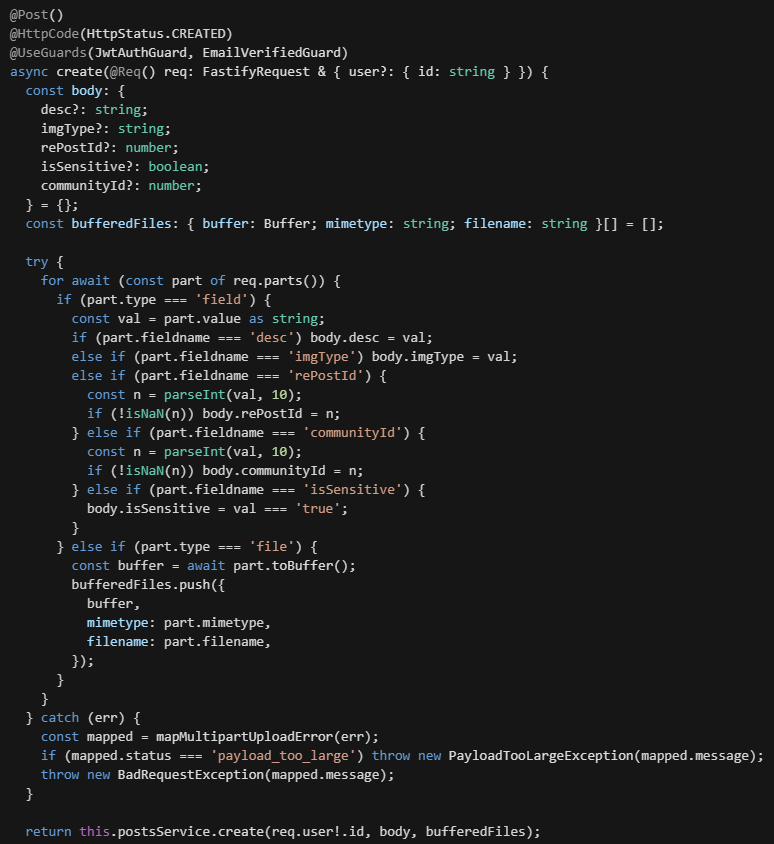
\includegraphics[width=0.92\linewidth,height=0.82\textheight,keepaspectratio]{images/image42.png}
  \caption{Code Snippet -- Post Management}
  \label{fig:36}
\end{figure}

\textbf{Service (Business Logic):} Executes post insertion and handles automatic hashtag discovery. It uses an ES6 RegExp matchAll(/\#([a-zA-Z0-9\_]+)/g) search to isolate tags, eliminate duplicate entries using a Set, and executes concurrent database upsert queries inside a Promise.all block. This establishes hashtag records and many-to-many relationship rows in SQL in a single non-blocking execution block.
\begin{figure}[H]
  \centering
  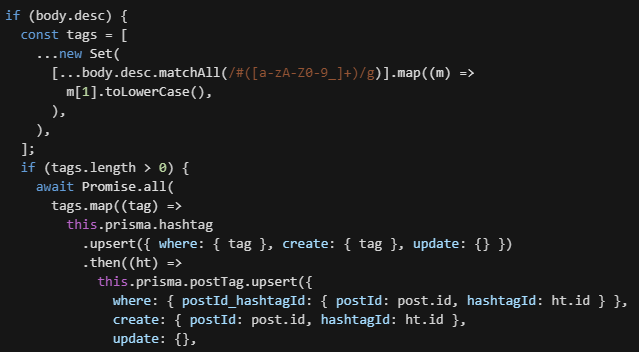
\includegraphics[width=0.92\linewidth,height=0.82\textheight,keepaspectratio]{images/image43.png}
  \caption{Code Snippet -- Post Management}
  \label{fig:37}
\end{figure}

\subsection{Module 4: Post Interaction}

\textbf{Controller (API Routes):} Exposes retrieval routes for comment feeds, integrates NestJS ParseIntPipe to sanitize and cast the parameter postId from a raw string into an integer directly at the controller routing layer, blocking malformed input types before database querying.
\begin{figure}[H]
  \centering
  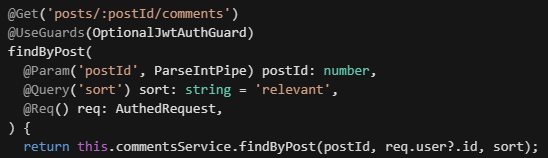
\includegraphics[width=0.92\linewidth,height=0.82\textheight,keepaspectratio]{images/image44.png}
  \caption{Code Snippet -- Post Interaction}
  \label{fig:38}
\end{figure}

\textbf{Service (Business Logic):} Resolves threaded nested hierarchical comment streams. The service executes recursive queries through Prisma, retrieving top-level parent comments and nesting subsequent children (replies) up to 5 levels deep. Root replies are sorted dynamically according to popularity (like count) or recency, while inner child replies are sorted chronologically (createdAt: asc) to maintain coherent thread conversations.
\begin{figure}[H]
  \centering
  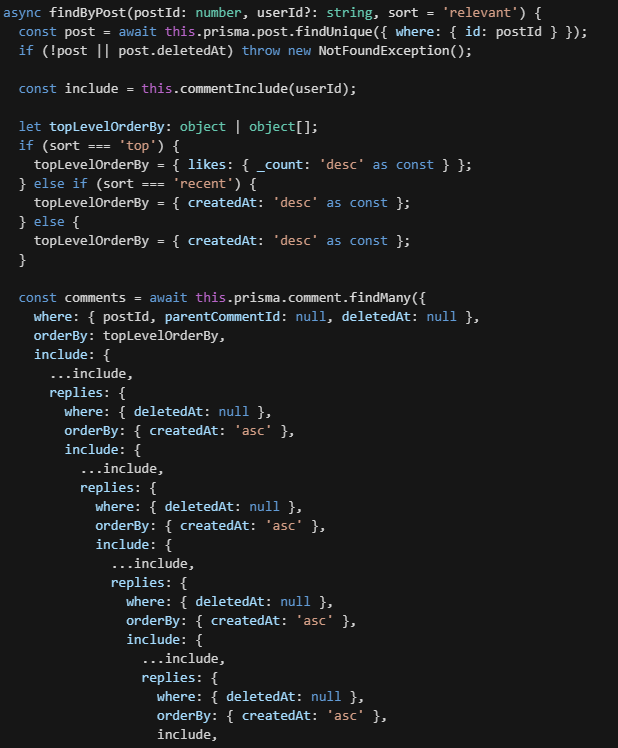
\includegraphics[width=0.92\linewidth,height=0.82\textheight,keepaspectratio]{images/image45.png}
  \caption{Code Snippet -- Post Interaction}
  \label{fig:39}
\end{figure}

\subsection{Module 5: User Relationship Management}

\textbf{Controller (API Routes):} Endpoint that handles user blocks. Combines session validation (JwtAuthGuard) and security moderation checks (BannedUserGuard) to prevent blocked or banned users from initiating relationship modifications on the platform.
\begin{figure}[H]
  \centering
  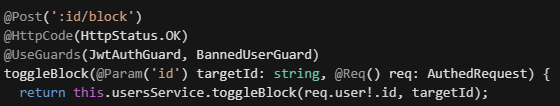
\includegraphics[width=0.92\linewidth,height=0.82\textheight,keepaspectratio]{images/image46.png}
  \caption{Code Snippet -- User Relationship Management}
  \label{fig:40}
\end{figure}

\textbf{Service (Business Logic):} Implements bidirectional blocking logic. When a block is established, the database removes mutual follow instances in a unified transaction (deleteMany). Cache invalidation commands are pushed immediately to Redis to delete old relationship state graphs (graph:follows and graph:blockedPeers), enforcing instant privacy boundaries on subsequent page requests.
\begin{center}
  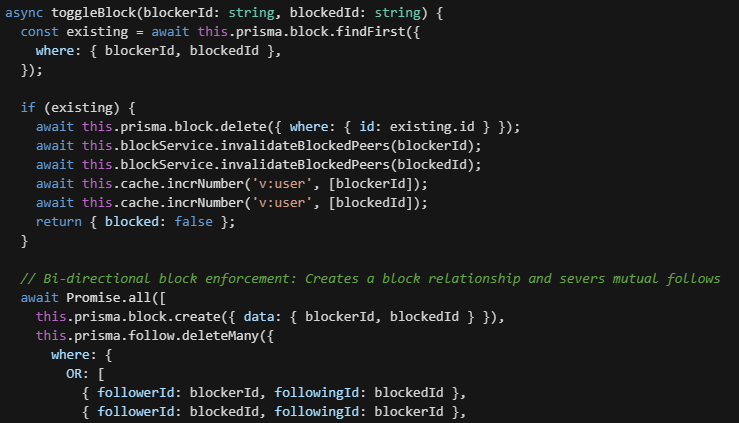
\includegraphics[width=0.92\linewidth,height=0.82\textheight,keepaspectratio]{images/image47.png}
\end{center}
\begin{figure}[H]
  \centering
  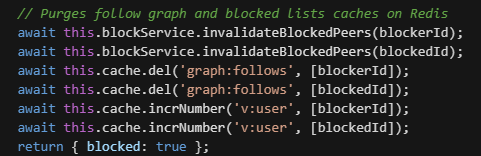
\includegraphics[width=0.92\linewidth,height=0.82\textheight,keepaspectratio]{images/image48.png}
  \caption{Code Snippet -- User Relationship Management}
  \label{fig:41}
\end{figure}

\subsection{Module 6: Profile Management}

\textbf{Controller (API Routes):} Defines routes for loading specific user profiles. Uses the OptionalJwtAuthGuard to verify session parameters, allowing guests to read profiles while letting authenticated users pass search queries (q) and tab queries.
\begin{figure}[H]
  \centering
  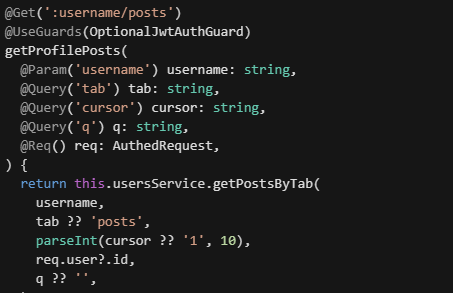
\includegraphics[width=0.92\linewidth,height=0.82\textheight,keepaspectratio]{images/image49.png}
  \caption{Code Snippet -- Profile Management}
  \label{fig:42}
\end{figure}

\textbf{Service (Business Logic):} Dynamically compiles PostgreSQL where conditions are based on selected categories (media, likes, posts). Security checks are enforced inside the service (isBlockedPair) to verify blocking status before compiling profile content, blocking malicious API requests from bypass attempts.
\begin{center}
  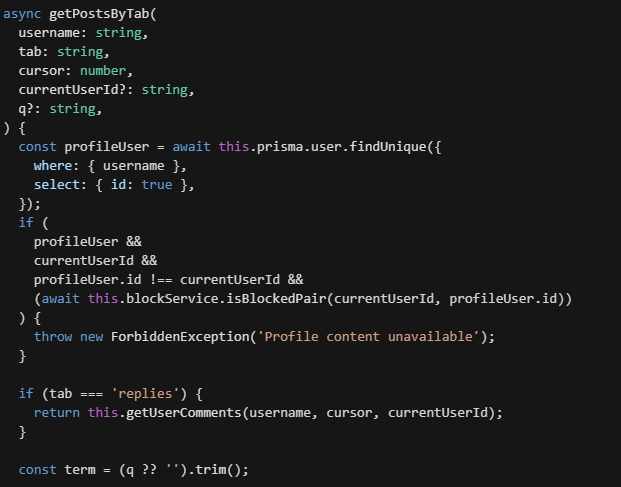
\includegraphics[width=0.92\linewidth,height=0.82\textheight,keepaspectratio]{images/image50.png}
\end{center}
\begin{center}
  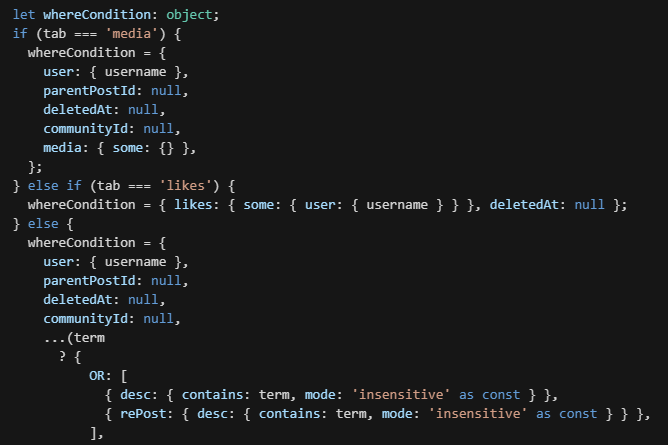
\includegraphics[width=0.92\linewidth,height=0.82\textheight,keepaspectratio]{images/image51.png}
\end{center}
\begin{figure}[H]
  \centering
  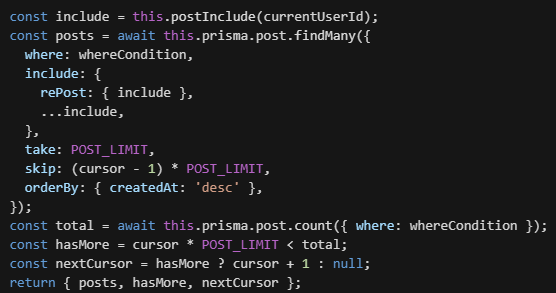
\includegraphics[width=0.92\linewidth,height=0.82\textheight,keepaspectratio]{images/image52.png}
  \caption{Code Snippet -- Profile Management}
  \label{fig:43}
\end{figure}

\subsection{Module 7: Direct Messaging}

\textbf{Controller (API Routes):} Routing endpoint for message dispatching. Guarded by the EmailVerifiedGuard to restrict real-time communication privileges to verified users, preventing malicious spam and automated bot registration flows.
\begin{figure}[H]
  \centering
  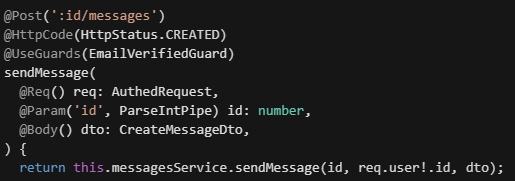
\includegraphics[width=0.92\linewidth,height=0.82\textheight,keepaspectratio]{images/image53.png}
  \caption{Code Snippet -- Direct Messaging}
  \label{fig:44}
\end{figure}

\textbf{Service (Business Logic):} Encapsulates message creation and conversation metadata updates within an ACID \$transaction block. Once changes are successfully written to SQL, the service leverages Socket.io WebSocket Gateway to broadcast the message payload (newMessage event) to the recipient's secure connection channel, subsequently invalidating the unread count in Redis.
\begin{center}
  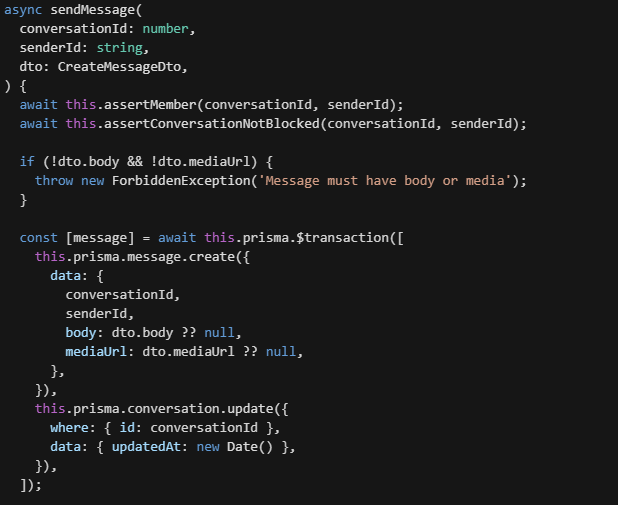
\includegraphics[width=0.92\linewidth,height=0.82\textheight,keepaspectratio]{images/image54.png}
\end{center}
\begin{figure}[H]
  \centering
  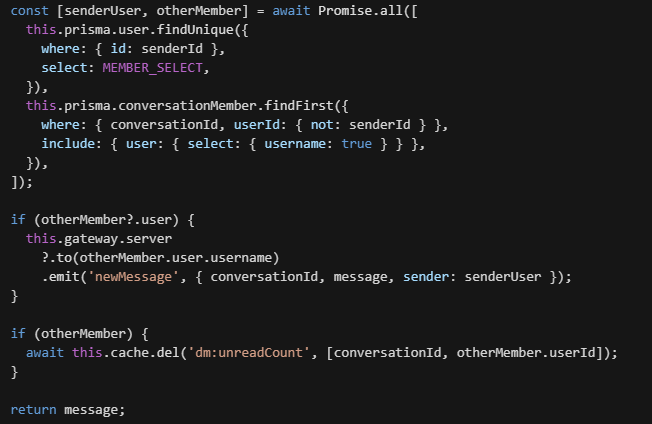
\includegraphics[width=0.92\linewidth,height=0.82\textheight,keepaspectratio]{images/image55.png}
  \caption{Code Snippet -- Direct Messaging}
  \label{fig:45}
\end{figure}

\subsection{Module 8: Real-time Notifications}

\textbf{Controller (API Routes):} Handlers request for reading the authenticated user's notification log history, supporting paging via integer cursors and filters for read/unread notification states.
\begin{figure}[H]
  \centering
  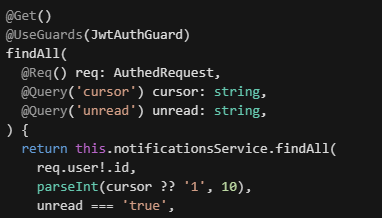
\includegraphics[width=0.92\linewidth,height=0.82\textheight,keepaspectratio]{images/image56.png}
  \caption{Code Snippet -- Real-time Nofications}
  \label{fig:46}
\end{figure}

\textbf{WebSocket Gateway (Real-time Hub):} Implements a full-duplex WebSocket hub powered by Socket.io. It integrates @socket.io/redis-adapter to enable cluster pub/sub synchronization, allowing horizontal scaling of backend instances. It reads the incoming handshake headers to fetch the breadit\_session cookie, validation-checking the JWT signature before establishing the connection.
\begin{figure}[H]
  \centering
  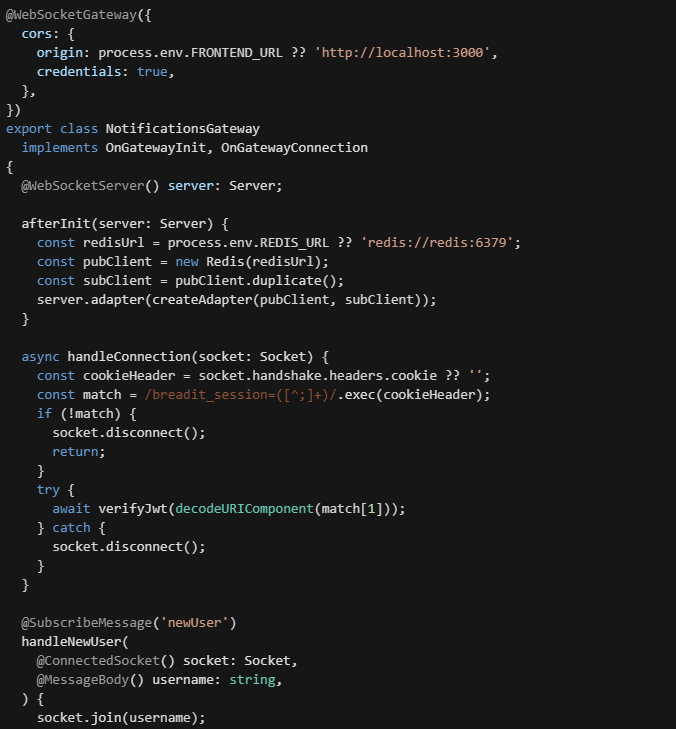
\includegraphics[width=0.92\linewidth,height=0.82\textheight,keepaspectratio]{images/image57.png}
  \caption{Code Snippet -- Real-time Nofications}
  \label{fig:47}
\end{figure}

\subsection{Module 9: Community Management}

\textbf{Controller (API Routes):} Exposes endpoint for community moderators to approve or reject pending member posts, validating basic request parameters (id and postId format) before calling the Service layer.
\begin{figure}[H]
  \centering
  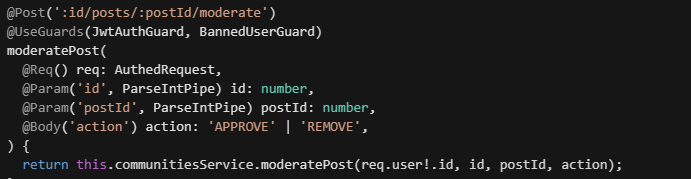
\includegraphics[width=0.92\linewidth,height=0.82\textheight,keepaspectratio]{images/image58.png}
  \caption{Code Snippet -- Community Management}
  \label{fig:48}
\end{figure}

\textbf{Service (Business Logic):} Implements community-level role-based access control (RBAC). The member's moderator/owner status in PostgreSQL before update the target post's isApproved flag. Posts trigger async notifications (COMMUNITY\_NEW\_POST) dispatched concurrently to all community members via Promise.all.
\begin{figure}[H]
  \centering
  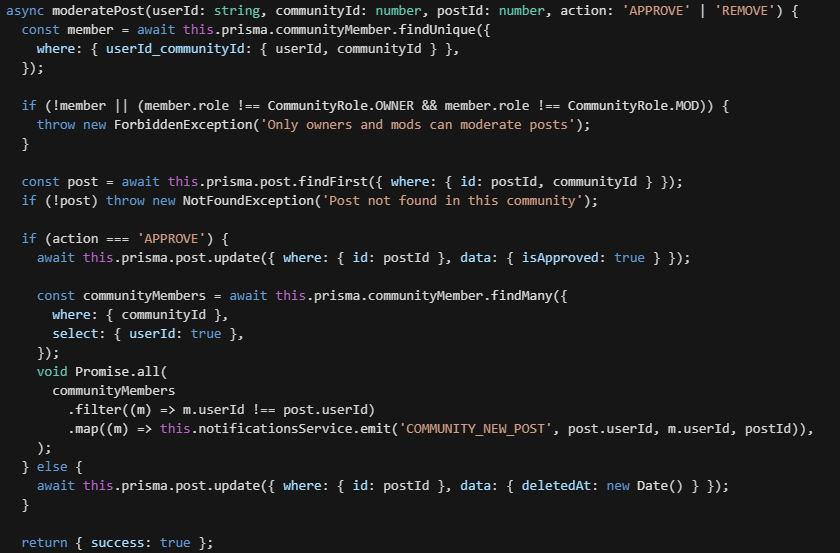
\includegraphics[width=0.92\linewidth,height=0.82\textheight,keepaspectratio]{images/image59.png}
  \caption{Code Snippet -- Community Management}
  \label{fig:49}
\end{figure}

\subsection{Module 10: Administrative Moderation}

\textbf{Controller (API Routes):} Controller endpoint for global moderation. Access is restricted by using global guards (RolesGuard) to verify that the executing account holds a site-wide role of 'ADMIN' before processing bans.
\begin{figure}[H]
  \centering
  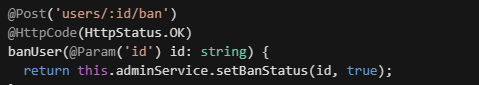
\includegraphics[width=0.92\linewidth,height=0.82\textheight,keepaspectratio]{images/image60.png}
  \caption{Code Snippet -- Administrative Moderation}
  \label{fig:50}
\end{figure}

\textbf{Service (Business Logic}\textbf{)}: Updates a user account's banned state in PostgreSQL. Ensure instant moderation enforcement, the service immediately emits an accountBanned event to the user's active WebSocket room. The client-side application listens for this event to clear session state, revoke cookies, and force redirect the user to prevent the interaction.
\begin{figure}[H]
  \centering
  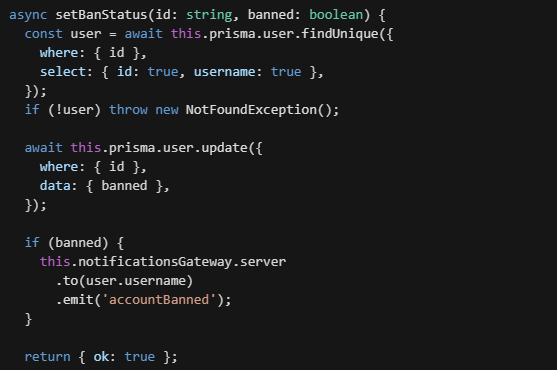
\includegraphics[width=0.92\linewidth,height=0.82\textheight,keepaspectratio]{images/image61.png}
  \caption{Code Snippet -- Administrative Moderation}
  \label{fig:51}
\end{figure}

\section{Frontend Implementation}

The frontend application of Breadit serves as the interactive presentation layer. It is built using the Next.js 15 framework and follows component-based architecture. Client-side state and caching are managed using TanStack React Query, while routing and route guards are handled through Next.js App Router and server-side middleware, ensuring a responsive and seamless user experience.

\subsection{Authentication \& Onboarding Flow (/sign-up, /sign-in, /verify)}
\begin{itemize}
  \item Regex-based Client Validation: During user registration, the system validates the email format instantly in real-time (onChange) utilizing the validateEmail function and a custom regular expression (EMAIL\_RE). This provides instant visual feedback to the user, preventing unnecessary HTTP requests to the backend API.
  \item Stateful Query Parameter Interception: The Login component reads URL query parameters (verified, reset, ban	ned) to dynamically display administrative status alerts (such as informing banned users of account suspension).
  \item OTP Submission Flow: Upon successful registration, the client routes the user to the OTP page. The component enforces a strict 6-digit numeric pattern verification (pattern="[0-9]\{6\}" and inputMode="numeric") before enabling form submission. It invokes the verification API asynchronously and redirects the user to the login screen with a success query parameter upon approval.
\end{itemize}
\begin{figure}[H]
  \centering
  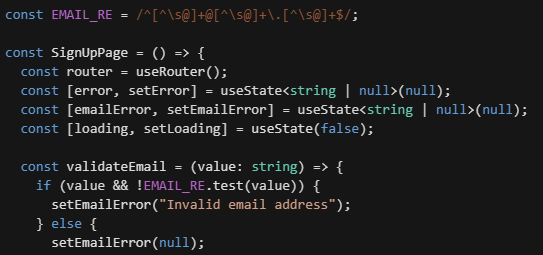
\includegraphics[width=0.92\linewidth,height=0.82\textheight,keepaspectratio]{images/image62.png}
  \caption{Code Snippet -- Sign-Up Page}
  \label{fig:52}
\end{figure}
\begin{figure}[H]
  \centering
  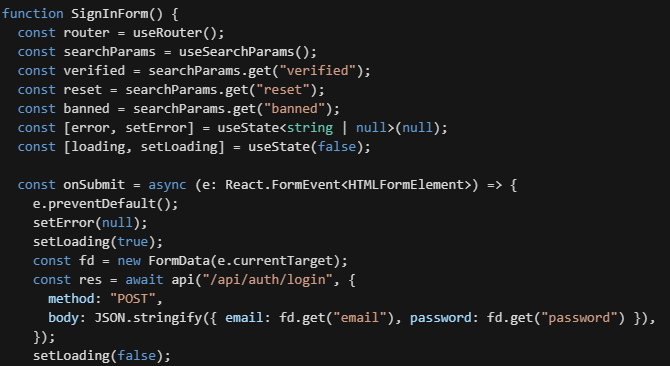
\includegraphics[width=0.92\linewidth,height=0.82\textheight,keepaspectratio]{images/image64.png}
  \caption{Code Snippet -- Sign-In Page}
  \label{fig:53}
\end{figure}
\begin{figure}[H]
  \centering
  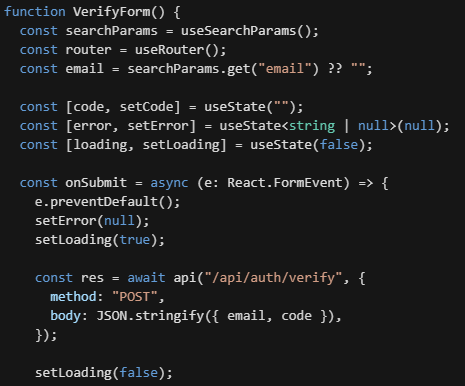
\includegraphics[width=0.92\linewidth,height=0.82\textheight,keepaspectratio]{images/image65.png}
  \caption{Code Snippet -- Verify Page}
  \label{fig:54}
\end{figure}

\subsection{Main Feed \& Discovery Page (/ - Home \& Explore Feed)}
\begin{itemize}
  \item URL-Driven Tabs: The / (Home) route parses the URL search parameters to retrieve the specific active feed type (For you, Explore, Following, Communities). This value is passed down to the Feed wrapper.
  \item useInfiniteQuery Integration: The client-side logic leverages TanStack's useInfiniteQuery hook. By specifying an initial page parameter of 1, the client fetches post items asynchronously. The query key depends on the active tab and filters (userProfileId, feed, communityId), enabling independent cache for each view.
  \item Cursor-based Pagination \& Scroll Trigger: The API returns a nextCursor value. The hook reads this via getNextPageParam to keep track of the subsequent page's cursor. The InfiniteScroll component monitors window scrolls parameters; when the user nears the page bottom, it triggers fetchNextPage, requesting the next page. This forms a smooth, Twitter-like feed scroll experience.
\end{itemize}
\begin{figure}[H]
  \centering
  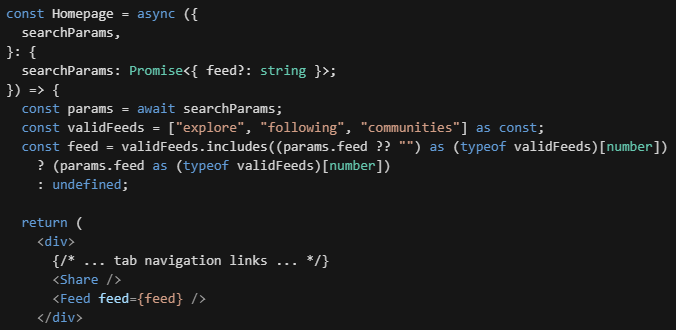
\includegraphics[width=0.92\linewidth,height=0.82\textheight,keepaspectratio]{images/image66.png}
  \caption{Code Snippet -- Feed Routing Layout}
  \label{fig:55}
\end{figure}
\begin{center}
  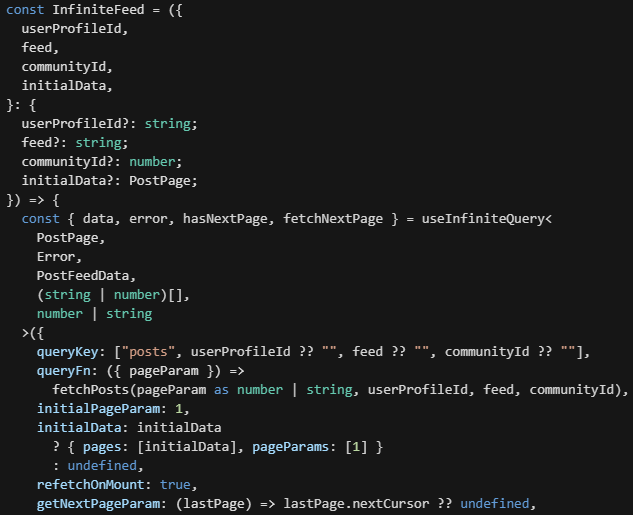
\includegraphics[width=0.92\linewidth,height=0.82\textheight,keepaspectratio]{images/image67.png}
\end{center}
\begin{figure}[H]
  \centering
  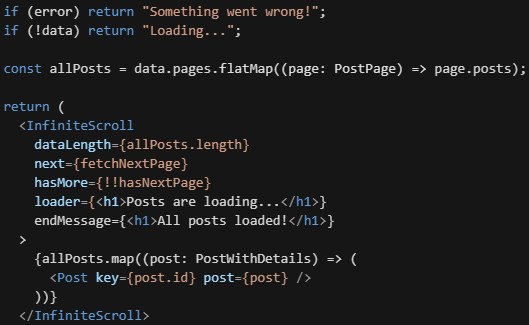
\includegraphics[width=0.92\linewidth,height=0.82\textheight,keepaspectratio]{images/image68.png}
  \caption{Code Snippet -- Main Home Page}
  \label{fig:56}
\end{figure}

\subsection{Direct Messaging \& Chat Interface (/messages)}
\begin{itemize}
  \item WebSocket Handshake and Session Security: The React client establishes a persistent connection with the NestJS Socket.io server, utilizing withCredentials: true to forward session credentials.
  \item Event-Driven Thread Updates: Inside MessageThread.tsx, the component registers event listeners. When the server emits a new message payload, the callback triggers immediately, modifying the TanStack React Query cache dynamically via queryClient.setQueryData to append the message to the view, and performing a smooth programmatic scroll to focus on the new message.
  \item Room-scoped Typing Broadcasts: The custom hook useTypingIndicator manages room-scoped typing indicators. Upon mount, the client joins a conversation room. Typing input textareas trigger onKeystroke(), which emits startTyping events and sets a 3-second debounce timer. If typing stops, stopTyping is emitted. Meanwhile, the client listens to incoming userTyping / userStopTyping events to display real-time feedback.
\end{itemize}
\begin{figure}[H]
  \centering
  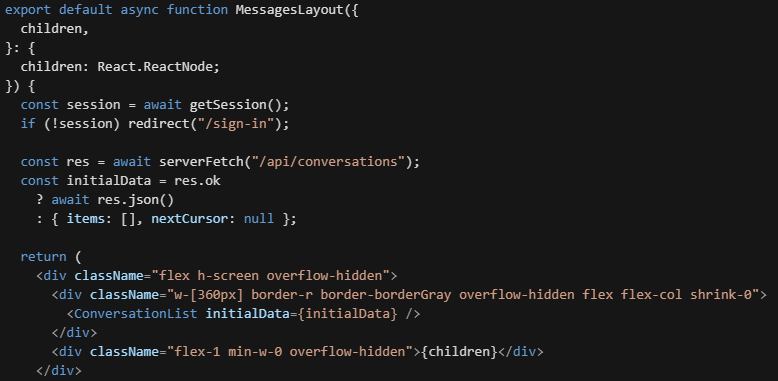
\includegraphics[width=0.92\linewidth,height=0.82\textheight,keepaspectratio]{images/image69.png}
  \caption{Code Snippet -- Messages Layout}
  \label{fig:57}
\end{figure}
\begin{figure}[H]
  \centering
  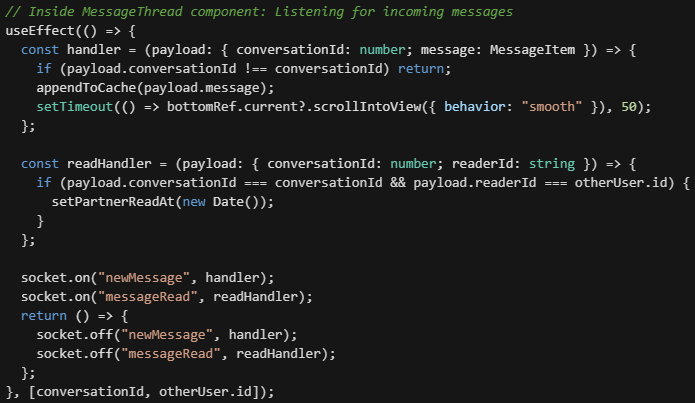
\includegraphics[width=0.92\linewidth,height=0.82\textheight,keepaspectratio]{images/image70.png}
  \caption{Code Snippet -- Real-time Message Thread}
  \label{fig:58}
\end{figure}
\begin{figure}[H]
  \centering
  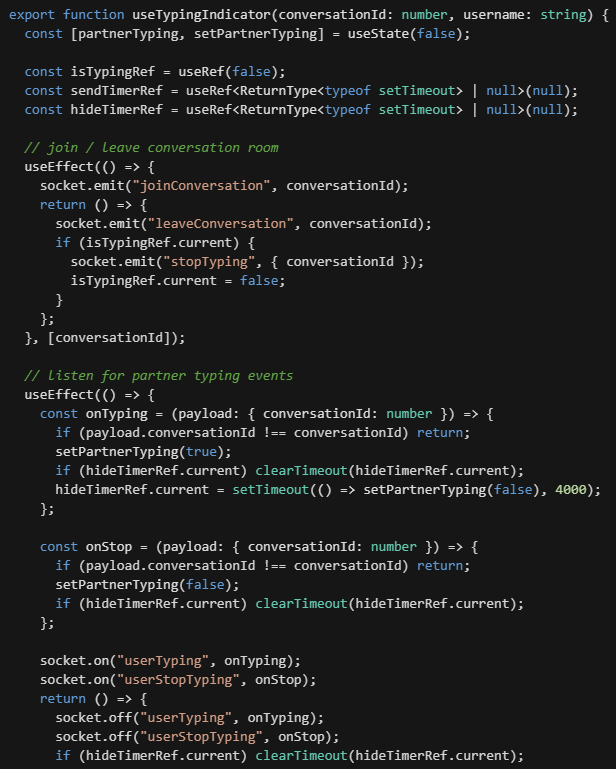
\includegraphics[width=0.92\linewidth,height=0.82\textheight,keepaspectratio]{images/image71.png}
  \caption{Code Snippet -- Typing Indicator Hook}
  \label{fig:59}
\end{figure}

\subsection{User Profile Page (/[username])}
\begin{itemize}
  \item Block-Aware Server Rendering: In [username]/page.tsx, the server performs a pre-fetch on the target user's details. If relationship flags (blockedYou or blockedByYou) are true, the page is flagged as profileRestricted, returning a localized privacy screen instead of sensitive details.
  \item Interactive Tabs: In ProfileTabs.tsx, the client switches between tab selections (posts, replies, media, likes). Updating the activeTab state changes the query key of useInfiniteQuery in ProfileTabFeed.tsx.
  \item Dynamic Query Invalidation: Changing the tab triggers a react-query cache reset and initiates a HTTP request targeting /api/users/\$\{username\}/posts?tab=\$\{activeTab\} with credentials. The component captures 403 Forbidden statuses to prevent restricted users from accessing api-sensitive details.
\end{itemize}
\begin{figure}[H]
  \centering
  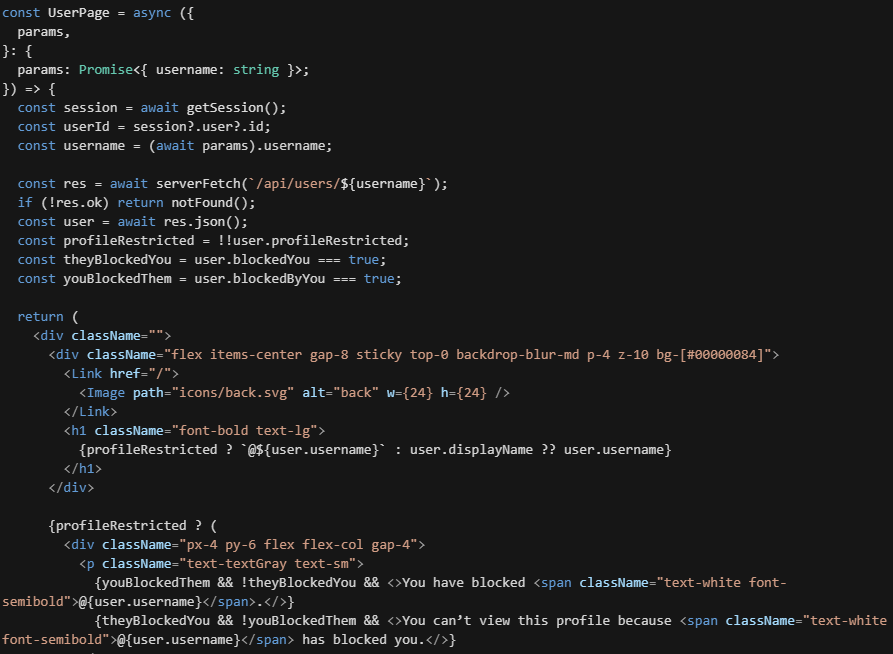
\includegraphics[width=0.92\linewidth,height=0.82\textheight,keepaspectratio]{images/image72.png}
  \caption{Code Snippet -- Server-Side Profile Page}
  \label{fig:60}
\end{figure}
\begin{figure}[H]
  \centering
  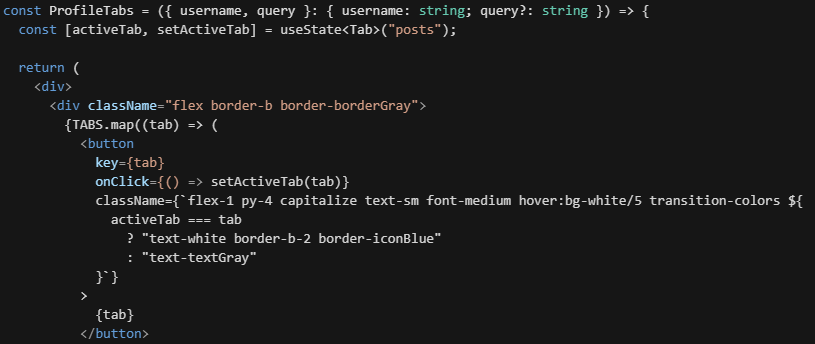
\includegraphics[width=0.92\linewidth,height=0.82\textheight,keepaspectratio]{images/image73.png}
  \caption{Code Snippet -- Profile Tab Switching}
  \label{fig:61}
\end{figure}
\begin{figure}[H]
  \centering
  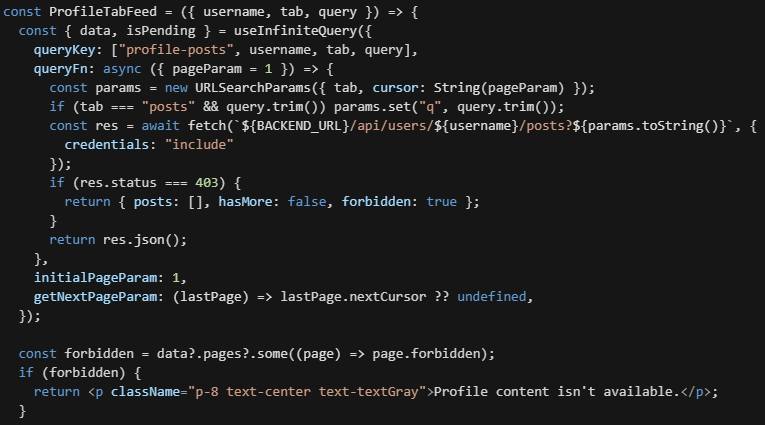
\includegraphics[width=0.92\linewidth,height=0.82\textheight,keepaspectratio]{images/image74.png}
  \caption{Code Snippet -- Profile Feed Fetcher}
  \label{fig:62}
\end{figure}

\subsection{Community Page (/c/[slug])}
\begin{itemize}
  \item Session-Forwarding Server Fetch: Next.js Server Components load the community config (getCommunity) on the server. By parsing cookies using cookies() and forwarding the JWT payload (breadit\_session) in headers, the backend determines membership roles prior to rendering the DOM, preventing unauthorized content leak.
  \item Optimistic State Updates: In CommunityHeader.tsx, the Join/Leave trigger uses a React Query mutation (useMutation). Upon success, it fires router.refresh(), triggering Next.js to re-verify server components and update UI labels dynamically.
  \item Role-Based Pending Queue (Moderator Queue): If the user is flagged as an OWNER or MOD, the page injects the PendingPostsBanner component. This fetch pending community posts from /api/communities/\$\{id\}/posts/pending and exposes instant Approve or Reject buttons. Moderation actions execute asynchronously, filtering out moderated posts instantly from the list.
\end{itemize}
\begin{figure}[H]
  \centering
  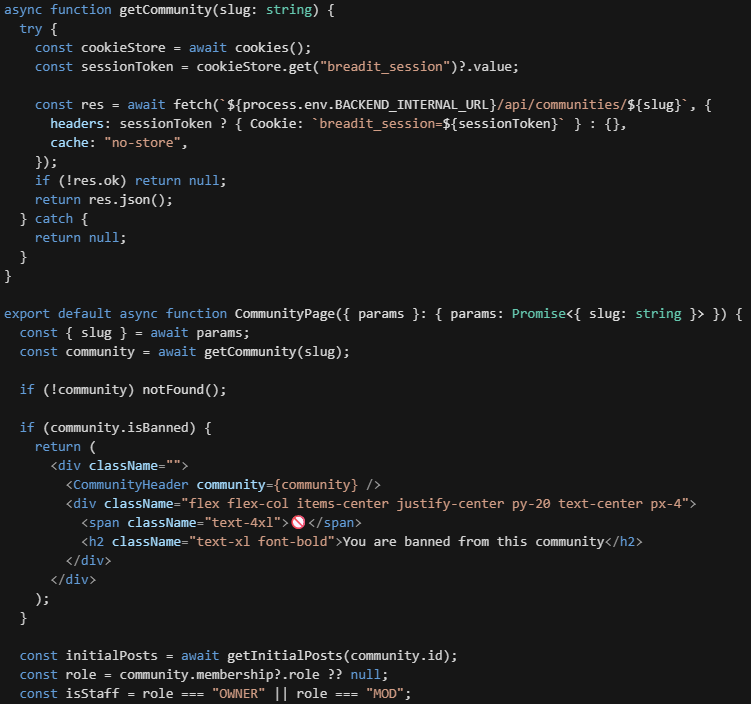
\includegraphics[width=0.92\linewidth,height=0.82\textheight,keepaspectratio]{images/image75.png}
  \caption{Code Snippet -- Community Server Component}
  \label{fig:63}
\end{figure}
\begin{figure}[H]
  \centering
  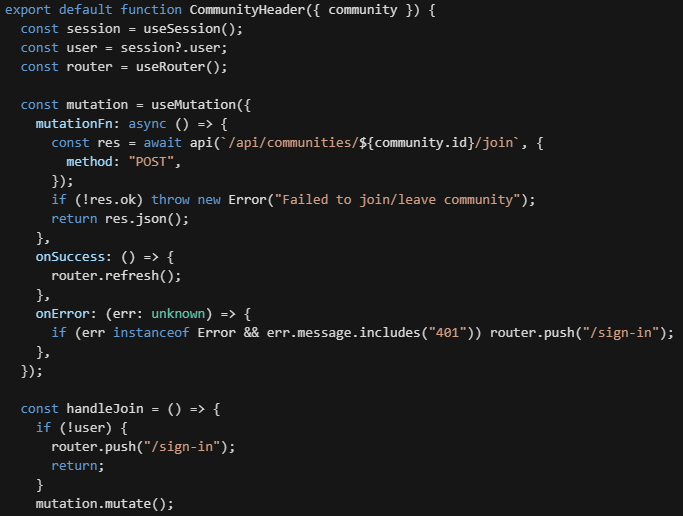
\includegraphics[width=0.92\linewidth,height=0.82\textheight,keepaspectratio]{images/image76.png}
  \caption{Code Snippet -- Join / Leave State}
  \label{fig:64}
\end{figure}
\begin{figure}[H]
  \centering
  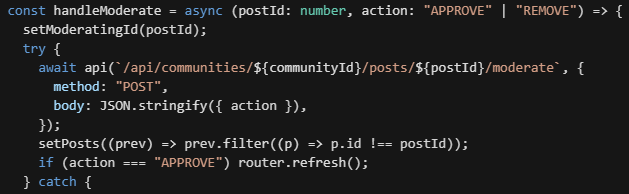
\includegraphics[width=0.92\linewidth,height=0.82\textheight,keepaspectratio]{images/image77.png}
  \caption{Code Snippet -- Moderator Pending Posts Queue}
  \label{fig:65}
\end{figure}

\subsection{Administrative Console (/admin-console)}
\begin{itemize}
  \item Server-Side Role Guarding: layout.tsx reads session details server-side. If the session is missing or the role claim is not equal to "ADMIN", the router triggers a prompt redirect (redirect("/")) before rendering any administrative markup.
  \item Global User Control (Ban/Unban): The UserTable displays a list of accounts. The administrator can click the Ban/Unban toggle, which calls the global ban endpoint. Triggering router.refresh() refreshes the table rows with the latest status.
  \item Content Report Resolution Queue (Report Queue): The ReportTable displays reported posts. It provides two operations: Dismissal (handleDismiss) which flags the report as clean and Delete Post (handleDeletePost) which removes the offending post from the system database.
\end{itemize}
\begin{figure}[H]
  \centering
  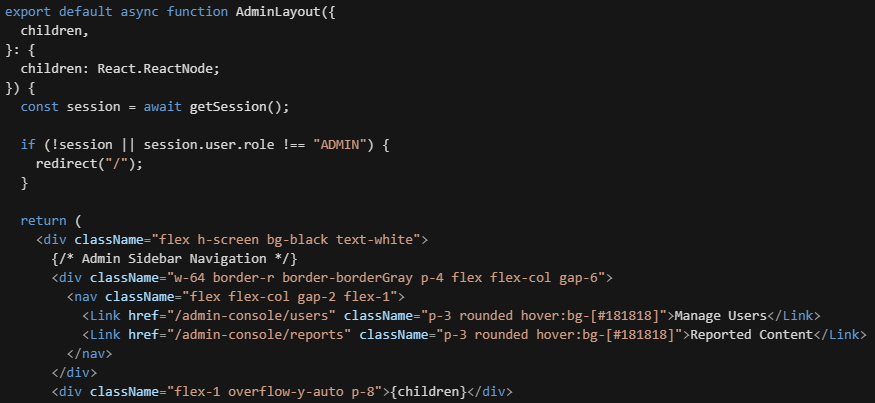
\includegraphics[width=0.92\linewidth,height=0.82\textheight,keepaspectratio]{images/image78.png}
  \caption{Code Snippet -- Administrative Layout}
  \label{fig:66}
\end{figure}
\begin{figure}[H]
  \centering
  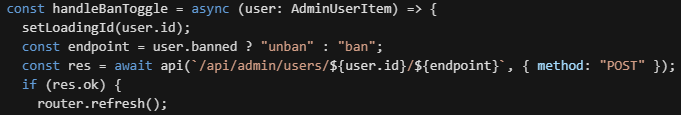
\includegraphics[width=0.92\linewidth,height=0.82\textheight,keepaspectratio]{images/image79.png}
  \caption{Code Snippet -- Banning Dashboard}
  \label{fig:67}
\end{figure}
\begin{figure}[H]
  \centering
  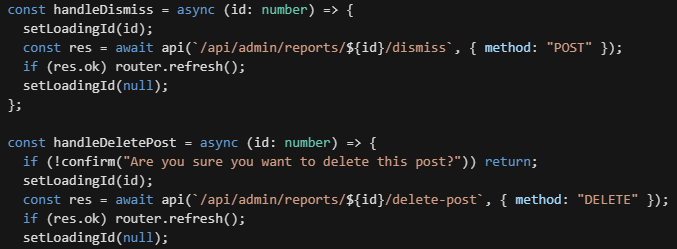
\includegraphics[width=0.92\linewidth,height=0.82\textheight,keepaspectratio]{images/image80.png}
  \caption{Code Snippet -- Report Queue}
  \label{fig:68}
\end{figure}
